\section{Building and Improving V1--V10}
\label{sec:development}
Our main tool for improvement was to observe \emph{where} a run first went wrong. A final count of five cookies does not say whether the remaining five were never grasped, lost during carrying, or placed in the wrong location. Each explanation calls for a different change. The advisor therefore requested stage-by-stage evidence; the executor tested a small fix and returned both successful and unsuccessful examples.

\subsection{V1--V5: from a basic idea to a tested policy}
The first four versions were development prototypes. They established the basic pipeline rather than a benchmark result for every version.

\paragraph{V1: a first closed-loop routine.}
We began with a geometric description of the robot, boxes, and expected cookie arrangement. The first controller estimated the scene from camera images and followed a sequence of approach, grasp, lift, carry, and release. It was capable of issuing real robot actions, but relied heavily on the nominal positions of the groups.

\paragraph{V2: look at the selected group.}
A broad estimate of all cookies was not enough for narrow grasping. We added a closer estimate of the actual group and a visual count of objects held between the fingers. This addressed two different questions: \emph{where should the gripper close?} and \emph{how many cookies did it take?}

\paragraph{V3: check camera alignment.}
A camera estimate can shift the perceived cookie position even when the robot motion is correct. We added a way to refine the front-camera alignment from visible source-box geometry. This aimed to reduce errors shared by all later steps.

\paragraph{V4: also inspect the target.}
A successful grasp is only half the job. The controller gained a target-side cookie count so that it could judge whether placement had made progress. This prepared the ground for later placement checks.

\paragraph{V5: first full frozen evaluation.}
V5 combined these pieces into a version that we tested on 20 seeds for each of six task/variation settings. Its mean completion rate was \textbf{46.83\%}, and official success was \textbf{14.17\%} (17/120). The failure logs were especially useful: the fingers often missed a narrow gap, failed to lift the entire group, or placed a partially held group against the target edge. Increasing the allowed action budget alone yielded little additional success, so the next versions focused on the quality of the movements.

\subsection{V6: use feedback where precision matters}
V6 was the largest early step forward. The executor worked on more accurate wrist-camera alignment, correct gripper-opening geometry, held-cookie measurements, and simpler recovery when a movement did not reach its goal. The advisor used small trials to identify errors in each stage before approving a wider evaluation.

One particularly useful result came from comparing two approaches to checking placement. A less restrictive version, which continued after reasonable visual evidence and kept uncertainty visible, succeeded in \textbf{19 of 45} development episodes. A version that insisted on strong visual confirmation before nearly every transition succeeded in only \textbf{3 of 45}. The stricter version often stopped because the camera could not see enough, even when movement was physically possible. We chose the less restrictive approach and retained the strict checker as diagnostic information.

In the paired 120-episode comparison at seeds 15000--15019, completion rose from \textbf{42.88\% to 74.58\%} and success from \textbf{5.83\% to 48.33\%}. This result gave a clear direction: improve local sensing and contact handling while allowing the robot to keep moving when it has sufficient evidence.

\subsection{V7: distinguish a helpful correction from a harmful one}
The next round targeted target-box localization and the last few millimeters of alignment. Some episodes improved sharply when the controller rejected an incorrect target estimate. However, the same correction sometimes displaced a previously successful approach. We tested reduced versions of the change instead of simply adding more recovery rules.

The paired comparison at seeds 16000--16019 found that V7 raised completion from \textbf{65.12\% to 67.38\%}, but official success changed from \textbf{36.67\% to 33.33\%}. This was a mixed result. We kept the improved observation and alignment ideas and carried the regressions into subsequent testing. The experience changed our review criterion: final quantity and official success had to be considered together, with specific attention to cases that were correct before a change.

\subsection{V8: separate the two tasks and handle the next move}
The two packing tasks need different handling. With ten cookies, the second group may be very small or very large, and the first group can block the next placement. V8 made it easier to give the two tasks distinct planning rules, observe the remaining source group after a change, and check the space that the moving fingers actually need.

An earlier controller could repeatedly attempt the same grasp without noticing that its information was stale. Another could choose a target point that was inside the box while the fingers could not safely withdraw. V8 began to address these task-level failures rather than treating them only as motion errors.

In the matched 17000-series evaluation, completion improved from \textbf{74.33\% to 81.21\%} and success from \textbf{45.00\% to 50.83\%}. The parent in this particular comparison was a composed candidate built from the previous work, not simply the published V7 folder. We preserved the exact parent and candidate code in the history archive.

\subsection{V9: make repeated pick-and-place reliable}
V9 focused on the long \pTen\ sequences. The most important lesson from the preceding runs was that correct motion on the first group did not guarantee progress on the third or fourth. The world had changed: a cookie had moved, an empty gap had appeared, or the target already contained a neighboring group.

The advisor proposed more specific source observations, clearer accounting of the remaining groups, better use of the visible box edges, and a distinction between a group that was physically in the target and one that passed every final scoring condition. Executors tested variations, measured regressions, and updated the controller only after a complete-run comparison.

A representative failure showed why this matters. After one group had been moved, the controller could continue searching for cookies in their old source position. More observation steps did not automatically help; the controller needed to update \emph{what had moved} and \emph{what still had to be done}. V9 improved this connection between observation, inventory, and the next action.

On seeds 19000--19019, V8 achieved \textbf{76.46\%} completion and \textbf{47.50\%} success; V9 achieved \textbf{88.12\%} completion and \textbf{75.00\%} success on those same settings. This established a more effective base for the final round.

\subsection{V10: selective fixes, then freeze}
For V10 we did not replace everything. We treated the six task/source cases as related but distinct problems and selected code that worked for each one. Important improvements included more reliable detection of the target box and already placed cookies, source-group re-identification after moving objects, more careful use of carried-object shape in collision checking, and better handling of a difficult final group.

A concrete example came from a source group that was carried successfully but also pulled an additional neighboring cookie. Although twenty cookies could appear in the target, the source-box condition still failed. This shifted our attention from merely increasing target count to protecting the remaining source cookies. Another example involved a target region mistakenly considered occupied because an old observation was reused. The solution was to revisit the evidence for that region, not blindly relax collision checks.

We also deliberately rejected changes that looked good on a few cases. A broad sideways correction briefly helped a four-case test. On a larger 127-case comparison it produced both new successes and \emph{fourteen lost previous successes}, with a small decrease in the total number of valid cookies. We did not merge this global correction into V10. Instead, we kept the stronger, better-tested components and used the failed examples to guide future targeted fixes.

The final V10 release is a frozen set of \textbf{78 policy runtime files}. We verified their hashes before formal testing. On seeds 24000--24019, the same-scene V9 baseline reached \textbf{94.96\%} completion and \textbf{89.17\%} success, while V10 reached \textbf{98.42\%} and \textbf{95.83\%}. Its final deployment uses the original task instructions and official scoring.

\begin{figure*}[t]
\centering
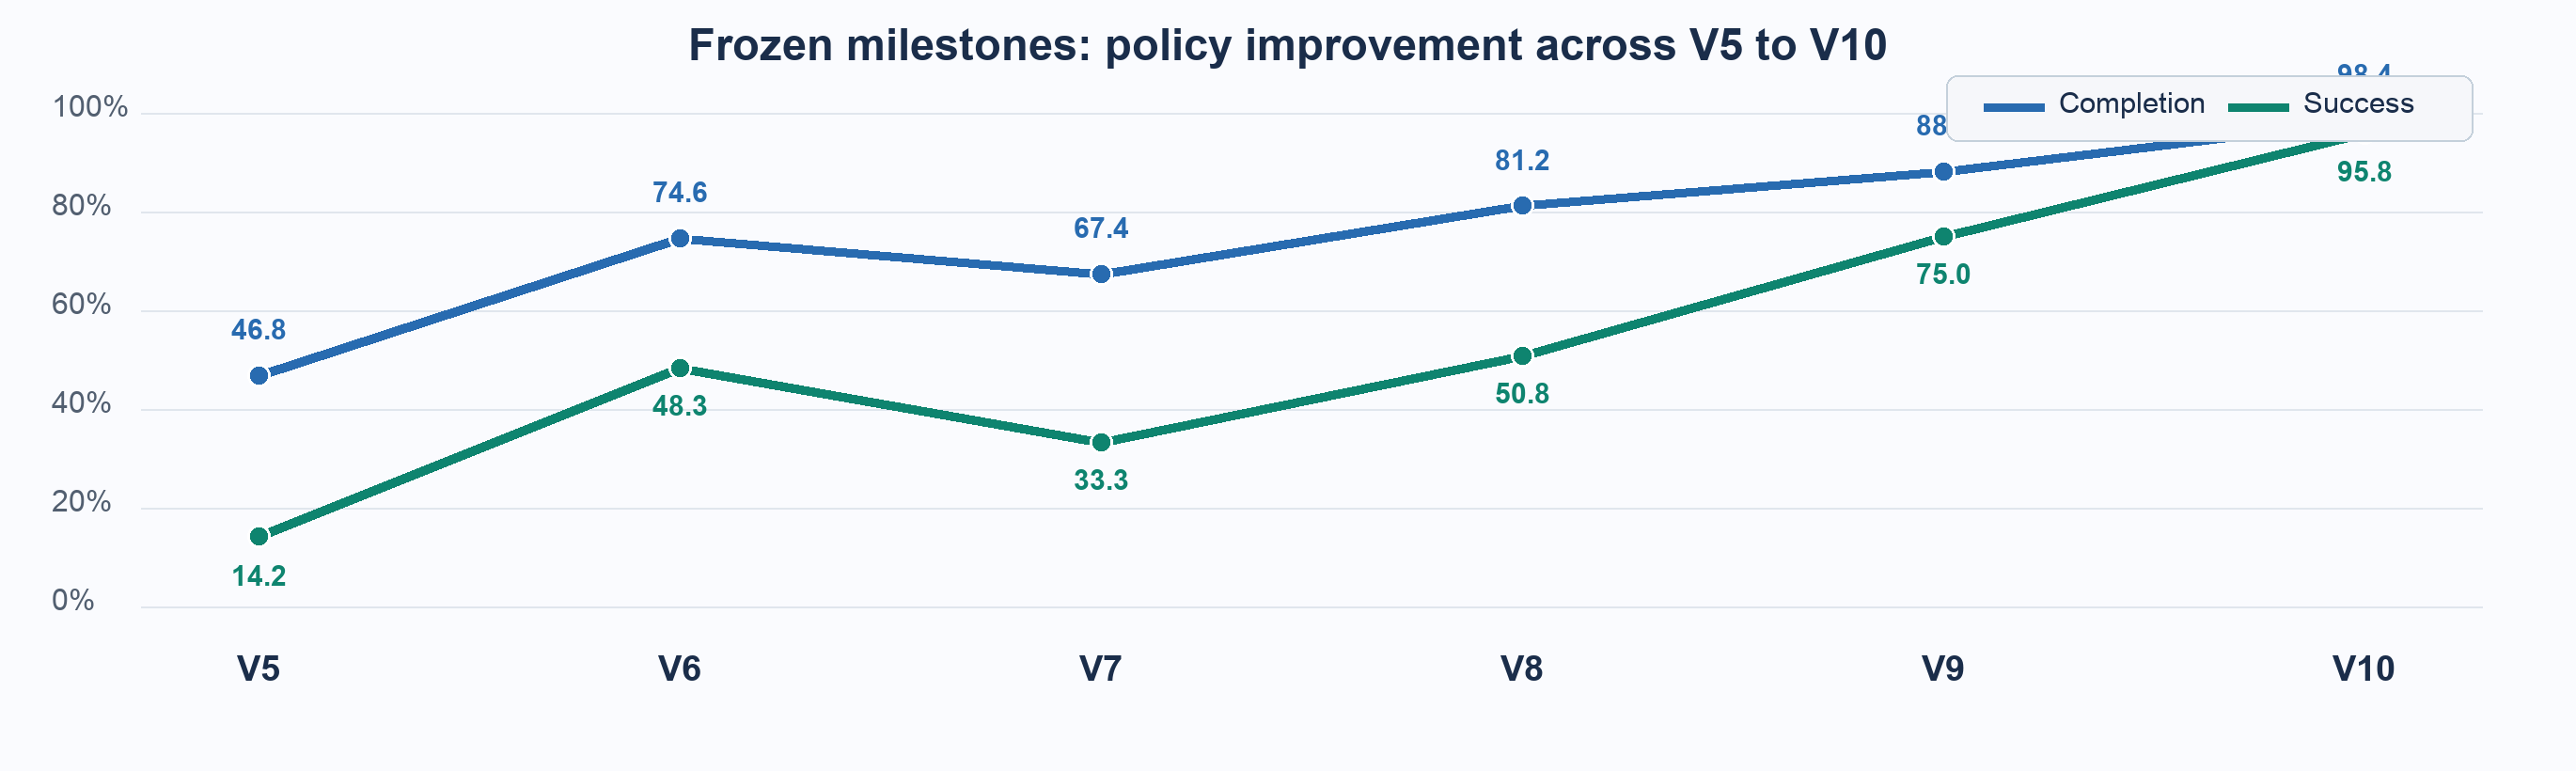
\includegraphics[width=0.99\textwidth]{figures/milestones.png}
\caption{The main milestones from V5 to V10, each measured on a newly chosen development or formal evaluation set. Values are mean completion and official success. Because the test scenes differ by round, Table~\ref{tab:paired} gives the more informative same-scene changes. The dips are retained rather than smoothed away.}
\label{fig:milestones}
\end{figure*}

\begin{table*}[t]
\centering\small
\caption{Same-scene comparisons used during selection. Each comparison has 120 episodes (20 seeds per setting); figures are mean completion and official success. Positive changes reflect paired improvements, while the V7 row illustrates a regression in one metric.}
\label{tab:paired}
\setlength{\tabcolsep}{3.7pt}\footnotesize\begin{tabular}{llrrrrrr}
\toprule
Test seeds & Old → new & Old completion & New completion & Change & Old success & New success & Change \\
\midrule
15000--15019 & V5 → V6 & 42.88\% & 74.58\% & +31.71 pp & 5.83\% & 48.33\% & +42.50 pp \\
16000--16019 & V6 → V7 & 65.12\% & 67.38\% & +2.25 pp & 36.67\% & 33.33\% & -3.33 pp \\
17000--17019 & Composed base → V8 & 74.33\% & 81.21\% & +6.88 pp & 45.00\% & 50.83\% & +5.83 pp \\
19000--19019 & V8 → V9 & 76.46\% & 88.12\% & +11.67 pp & 47.50\% & 75.00\% & +27.50 pp \\
24000--24019 & V9 → V10 & 94.96\% & 98.42\% & +3.46 pp & 89.17\% & 95.83\% & +6.67 pp \\
\bottomrule
\end{tabular}
\end{table*}

\paragraph{Our decision rule.}
Across these versions, a change was valuable when it improved complete tasks and did not needlessly spoil cases already handled well. We preferred small changes with a clear explanation to larger sets of emergency rules. A strong result on one scene could motivate a test, but wider same-scene comparisons decided whether it belonged in the frozen policy.
